% Especificaciones del tamaño de letra, tamaño de hoja, márgenes, librerias, etc.
\documentclass[12pt, letterpaper]{article}
\usepackage[english]{babel}
\usepackage{fancyhdr}
\usepackage[utf8]{inputenc}
\usepackage[T1]{fontenc}
\usepackage{amsmath}
\usepackage{graphicx}
\usepackage{subcaption}
\usepackage[hidelinks]{hyperref}
\usepackage{url}
\usepackage{amssymb}
\usepackage{float}
\usepackage[margin=1in]{geometry}
\usepackage{listings}
\usepackage{verbatim}
\renewcommand{\baselinestretch}{1.5}

% Enlace Bibliografía
\usepackage{csquotes}
\usepackage[notes,backend=biber]{biblatex-chicago}
\addbibresource{referencias.bib}

% Titulo, autores, fecha.
\title{Práctica \#3: Derivada Direccional, Distribuciones de Presión y Esfuerzo Cortante}
\author{Carlos A. Vásquez Castañeda \and 1155057 \and Grupo 395}
\date{Marzo 14, 2020}
\pagestyle{fancy}
\fancyhf{}
\rhead{Mecánica de Sustentación}
\lhead{Práctica \#3}
\rfoot{\thepage}


% Inicio del documento
\begin{document}
\maketitle

\section*{Introducción}
Las propiedades física de los sistemas como perfiles alares son de gran interés para conocer las posibilidades de sustentación de la geometría del perfil en cuestión. Si es posible contar con una expresión para la presión a la que es sometida la geometría, es posible calcular la variación de la presión en el espacio. Para lograr hacer esto, podemos utilizar el gradiente y esto nos otorgará un campo vectorial en donde los vectores apuntarán hacia los puntos donde se encuentre el cambio más alto. Sin embargo, en ocasiones es útil conocer el cambio de una propiedad en una dirección específica.

En el caso de las presiones, es posible calcular la presión que actúa sobre una geometría si podemos manipular la dirección en la que calculamos el gradiente. Este tipo de problemas son los que busca resolver la derivada direccional definida como:

\begin{equation}
	D_{\vec{v}}f = \nabla f \cdot \vec{v}
\end{equation}

Donde el vector $\vec{v}$ es el vector unitario apuntando en la dirección que es deseada. Es necesario que sea un vector unitario si no queremos cambiar el valor nominal de la derivada y así obtener los valores originales en cualquier dirección deseada.
\newpage

\section*{Procedimiento de la Práctica}
Empezaremos por el ejercicio dos ya que es el más sencillo y corto.
Para el ejercicio 2, donde se pide el trazo de los miembros "oficiales" de la familia NACA de 4 dígitos, se dan como miembros los siguientes conjuntos de parámetros:

\begin{equation}
	\begin{split}
		z_{máx} \in [0, 0.02, 0.04, 0.06] \\
		x_{mc} \in [0.2, 0.3, 0.4, 0.5, 0.6] \\
		t_{máx} \in [0.06, 0.09, 0.12, 0.15, 0.18, 0.21, 0.25] \\
	\end{split}
\end{equation}

Para realizar el trazado de la familia NACA con estos parámetros, necesitamos realizar una combinación de los mismos, para esto primeramente definimos los conjuntos.

\begin{figure}[H]
	\centering
	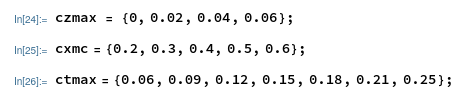
\includegraphics[width=\textwidth]{1.png}
	\caption{Declaración de los conjuntos con los parámetros antes mencionados.}
\end{figure}

Es posible realizar la combinación de los elementos de manera automática mediante la opción $Table$ como se muestra en la siguiente línea de código.

\begin{figure}[H]
	\centering
	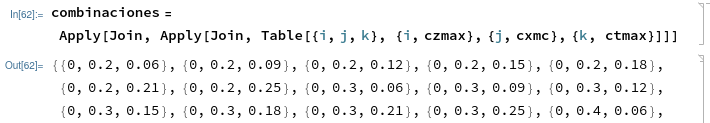
\includegraphics[width=\textwidth]{2.png}
	\caption{Combinaciones de los parámetros definidos.}
\end{figure}

La longitud de este arreglo se puede obtener mediante la función $Length$.
\begin{figure}[H]
	\centering
	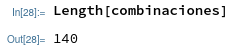
\includegraphics[width=0.6\textwidth]{3.png}
	\caption{140 combinaciones distintas obtenidas de los grupos mencionados anteriormente.}
\end{figure}

Finalmente podemos realizar el trazo de estos perfiles mediante la función $ParametricPlot$. En este ejemplo sólo se grafican los primeros 15 perfiles. En el archivo .nb se grafican los 140 perfiles.
\begin{figure}[H]
	\centering
	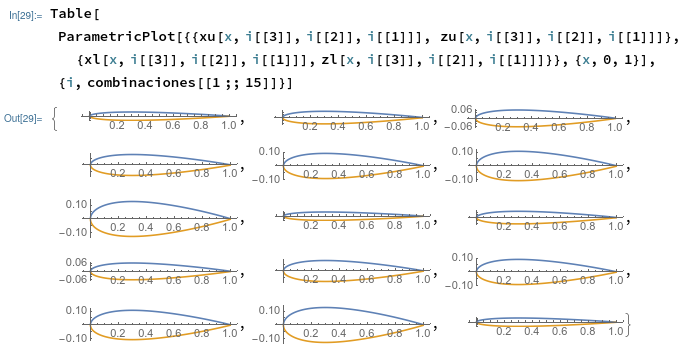
\includegraphics[width=0.9\textwidth]{4.png}
	\caption{Primeros 15 perfiles.}
\end{figure}

Ya listo el ejercicio 2, podemos proceder a realizar los siguientes ejercicios. Para realizar el trazo del perfil NACA6521 debemos definir los valores con anterioridad como se muestra a continuación.

\begin{figure}[H]
	\centering
	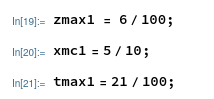
\includegraphics[width=0.5\textwidth]{5.png}
	\caption{Dimensiones de la NACA6521.}
\end{figure}

Con estos parámetros procedemos a graficar la parte superior e inferior del perfil alar.

\begin{figure}[H]
	\centering
	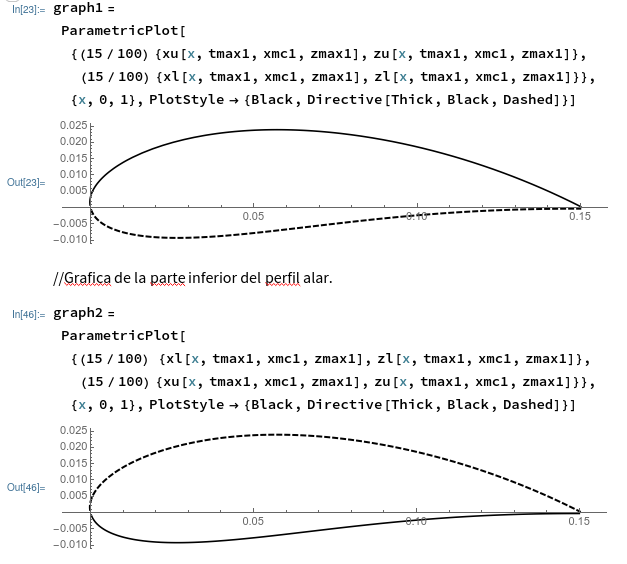
\includegraphics[width=0.8\textwidth]{6.png}
	\caption{Ambas superficies del perfil alar.}
\end{figure}

Ya dadas estas curvas, consideraremos solamente unos cuantos puntos para calcular la derivada direccional, por lo que realizaremos un arreglo que contenga veinticinco puntos normalizados.

\begin{figure}[H]
	\centering
	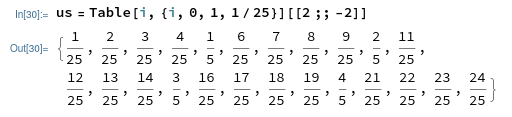
\includegraphics[width=\textwidth]{7.png}
	\caption{Arreglo de puntos normalizado.}
\end{figure}

\begin{figure}[H]
	\centering
	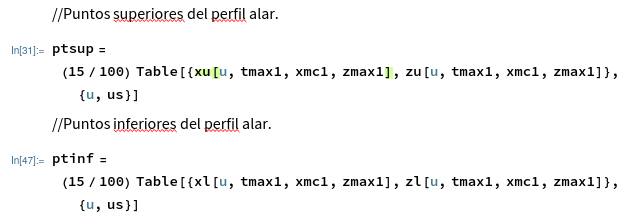
\includegraphics[width=\textwidth]{8.png}
	\caption{Puntos sobre las curvas dadas.}
\end{figure}


Pero no podemos realizar mucho sólo con estos puntos, así que lo siguiente que debemos realizar es definir la función de presión en el espacio y su gradiente.

\begin{figure}[H]
	\centering
	
\includegraphics[width=\textwidth]{9.png}
	\caption{Definición de la función de presión.}
\end{figure}

\begin{figure}[H]
	\centering
	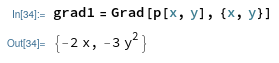
\includegraphics[width=\textwidth]{10.png}
	\caption{Cálculo del gradiente de la presión.}
\end{figure}

Con estos resultados es posible graficar la función de presiones junto a las curvas paramétricas y los puntos que hemos elegido a lo largo del perfil alar.

\begin{figure}[H]
	\centering
	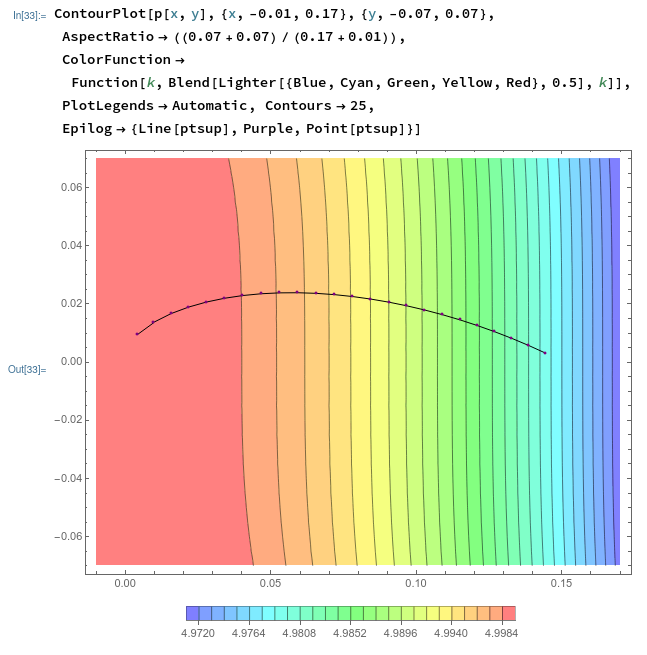
\includegraphics[width=0.85\textwidth]{11.png}
	\caption{Parte superior del perfil alar.}
\end{figure}

\begin{figure}[H]
	\centering
	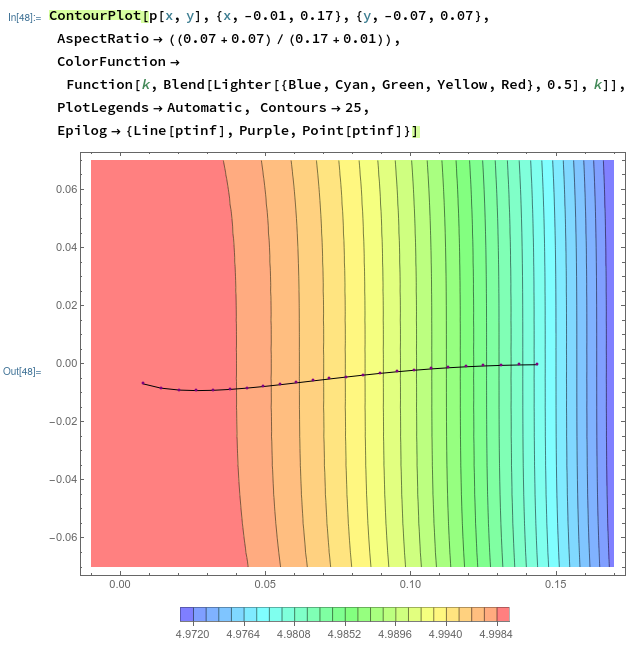
\includegraphics[width=0.85\textwidth]{12.png}
	\caption{Parte inferior del perfil alar.}
\end{figure}

Para lograr calcular la derivada direccional en los puntos deseados, es necesario calcular el gradiente en los puntos que hemos definido anteriormente.

\begin{figure}[H]
	\centering
	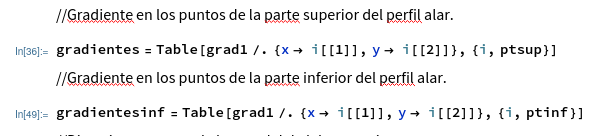
\includegraphics[width=\textwidth]{13.png}
	\caption{Gradiente en los distintos puntos del perfil alar.}
\end{figure}

Para encontrar la derivada direccional, la cual nos dará el cambio de presión en las direcciones que definamos (en este caso, normal a los puntos definidos), definimos el vector $u$ y se calcula la derivada direccional en toda la curva.

\begin{figure}[H]
	\centering
	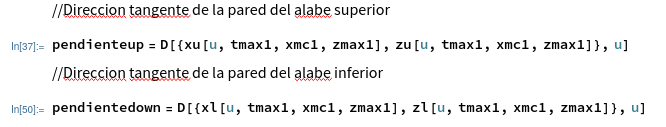
\includegraphics[width=\textwidth]{14.png}
	\caption{Direcciones tangentes.}
\end{figure}

Con esta información, es posible calcular los vectores normales y tangentes a la superficie del perfil, sin embargo lo haremos sólo con los puntos definidos anteriormente.

\begin{figure}[H]
	\centering
	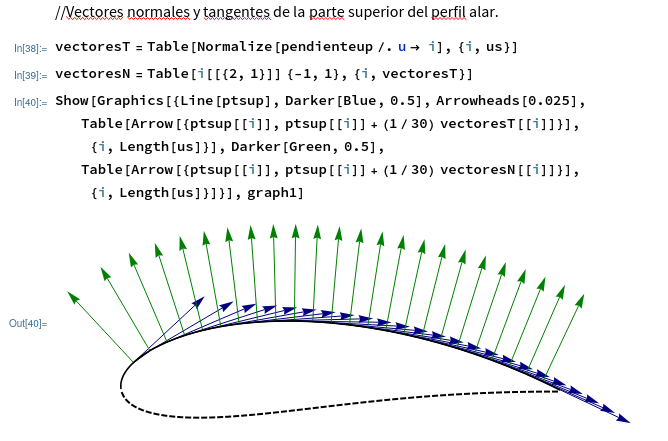
\includegraphics[width=\textwidth]{15.png}
	\caption{Vectores normales y tangentes a la superficie de la parte superior del perfil alar.}
\end{figure}

\begin{figure}[H]
	\centering
	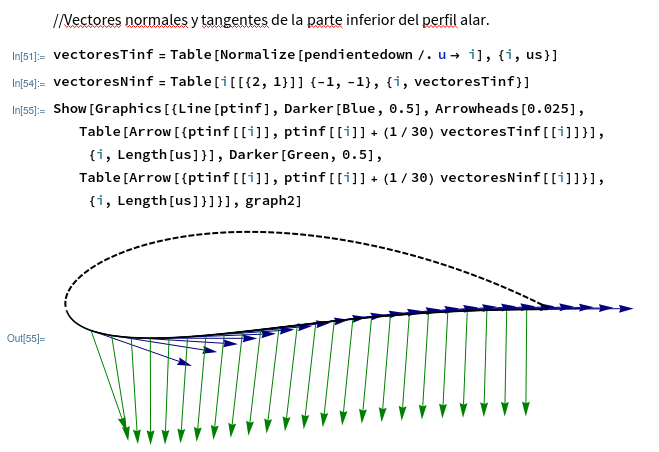
\includegraphics[width=\textwidth]{16.png}
	\caption{Vectores normales y tangentes a la superficie de la parte inferior del perfil alar.}
\end{figure}

Para analizar el valor de esfuerzos cortantes y presión a lo largo de la cuerda del perfil podemos poner en disposición los datos en una gráfica como se muestra a continuación.

\begin{figure}[H]
	\centering
	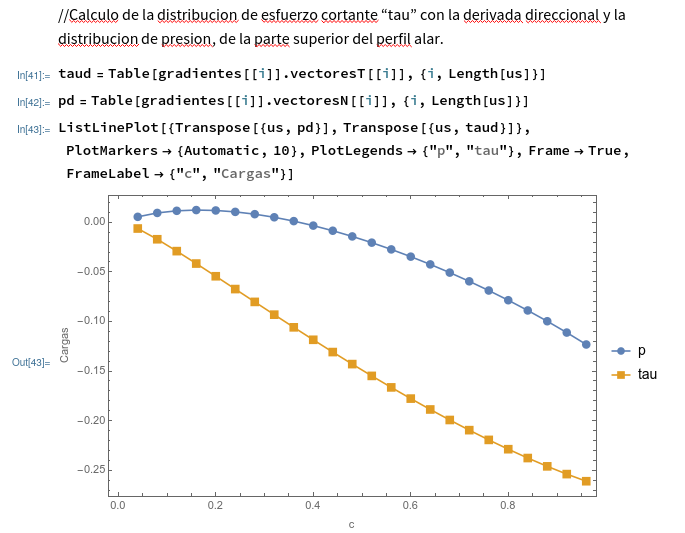
\includegraphics[width=0.7\textwidth]{17.png}
	\caption{Gráficas de esfuerzos cortantes y presión a lo largo de la cuerda superior.}
\end{figure}

\begin{figure}[H]
	\centering
	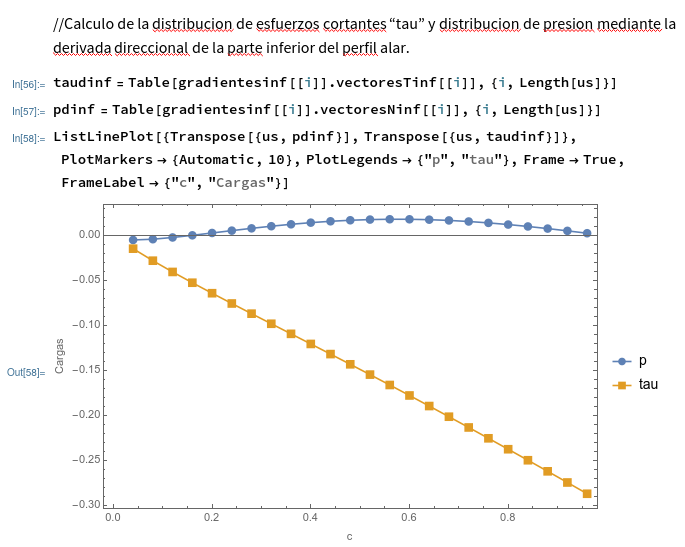
\includegraphics[width=0.7\textwidth]{18.png}
	\caption{Gráficas de esfuerzos cortantes y presión a lo largo de la cuerda inferior.}
\end{figure}

Los resultados de estas gräficas tienen sentido dado que la presión se espera que sea menor en la parte superior y mayor en la parte inferior, generando así la sustentación.

Por último, es posible disponer todos los resulados obtenidos en una tabla.

\begin{figure}[H]
	\centering
	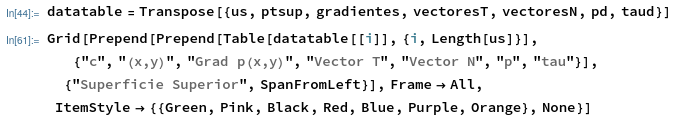
\includegraphics[width=\textwidth]{19.png}
	\caption{Código para generar la tabla.}
\end{figure}

\begin{figure}[H]
	\centering
	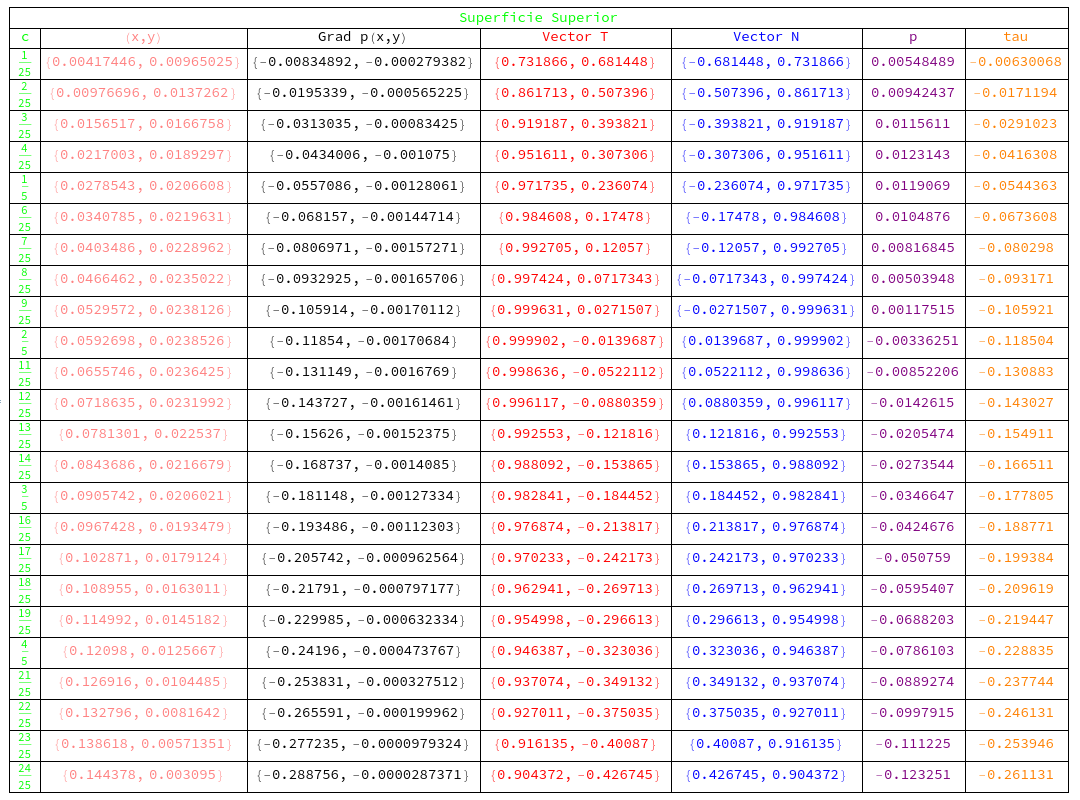
\includegraphics[width=\textwidth]{20.png}
	\caption{Datos de la parte superior.}
\end{figure}

\begin{figure}[H]
	\centering
	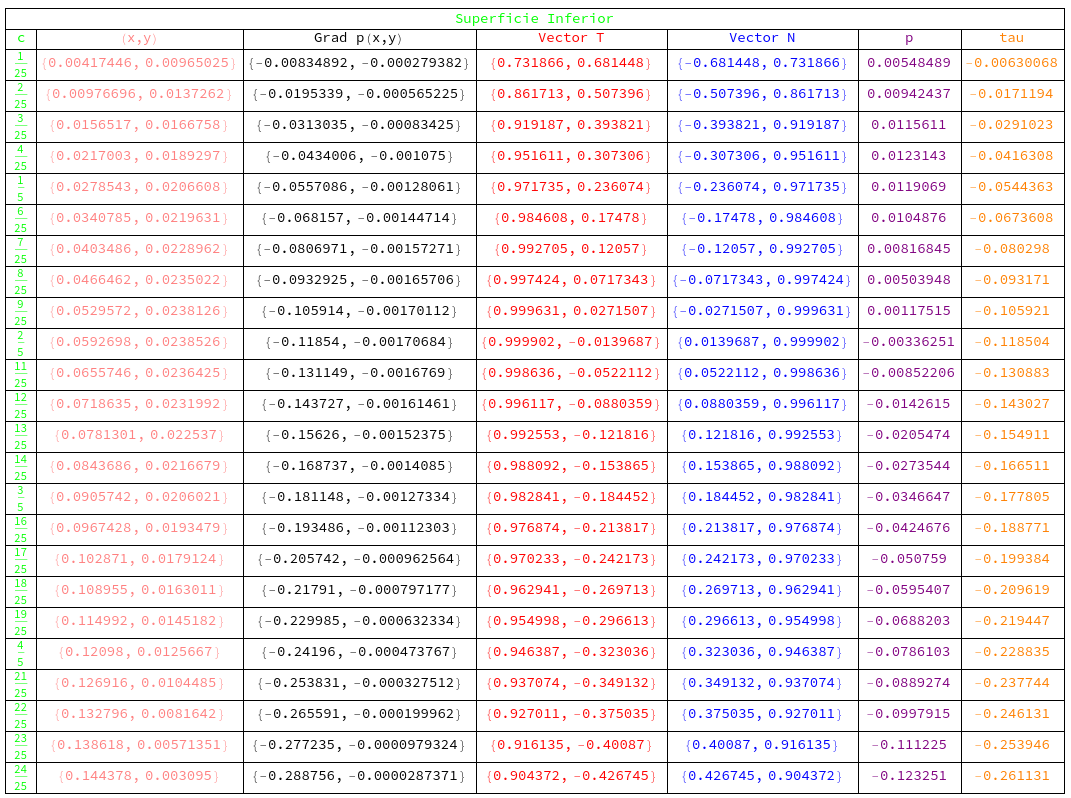
\includegraphics[width=\textwidth]{21.png}
	\caption{Datos de la parte inferior.}
\end{figure}

\section*{Conclusión}

Como hemos dicho anteriormente, los resultados de presión tienen sentido si lo que buscamos es la sustentación. La sustentación se obtiene cuando la diferencia de presiones permite que la fuerza neta actuando sobre el perfil alar sea positiva y éste se eleve. Esto se obtiene principalmente porque la trayectoria que tiene que recorrer el viento a lo largo del perfil alar es distinta para la parte inferior y superior, por lo tanto la parte superior se traslada a una velocidad mucho más alta, lo cual resulta en una presión más pequeña o negativa en la superficie superior, y en la superficie inferior es positiva o más grande.

En tanto a los esfuerzos cortantes, es esperado tener esfuerzos cortantes muchos más altos al inicio de la superficie del perfil alar debido al impacto del aire, y éste se regula y disminuye conforme la dirección del aire cambia cuando éste viaja a lo largo del perfil alar.
%%%%%  Bib
\renewcommand\refname{References}
\printbibliography
\end{document}
